\documentclass[12pt, oneside]{article}
\usepackage[letterpaper, margin=1in, headsep=0.5in]{geometry}
\usepackage[english]{babel}
\usepackage[utf8]{inputenc}
\usepackage{amsmath}
\usepackage{amsfonts}
\usepackage{amssymb}
\usepackage{tikz}
\usetikzlibrary{quotes, angles}
\usepackage{graphicx}
%\usepackage{pgfplots}
%\pgfplotsset{width=10cm,compat=1.9}
%\usepgfplotslibrary{statistics}
%\usepackage{pgfplotstable}
%\usepackage{tkz-fct}
%\usepackage{venndiagram}

\usepackage{fancyhdr}
\pagestyle{fancy}
\fancyhf{}
\rhead{\thepage \\Name: \hspace{1.5in}.\\}
\lhead{BECA / Dr. Huson / Geometry 10th Grade\\* Unit 2: Introduction to Proof\\5 November 2018}

\renewcommand{\headrulewidth}{0pt}

\begin{document}
\subsubsection*{Pre-Test: Trimester final exam}
  \vspace{0.5cm}
  \begin{enumerate}

\subsubsection*{Angle pairs: apply theorems, solve using algebra}

  \item Given the situation in the diagram, answer each question. Circle True or False. %\vspace{1cm}
      \begin{flushright}
      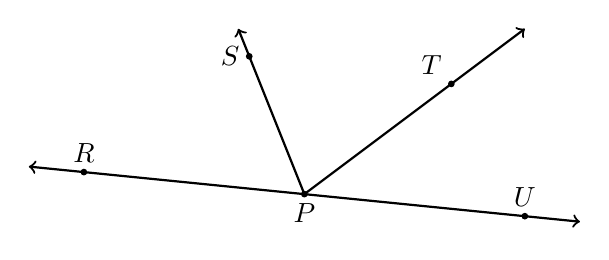
\begin{tikzpicture}[scale=0.7]
        \draw [->, thick] (0,0)--(4,3);
        \draw [<->, thick] (-5,.5)--(5,-.5);
        \draw [->, thick] (0,0)--(-1.2,3);
        \draw [fill] (-1,2.5) circle [radius=0.05] node[left ]{$S$};
        \draw [fill] (2.66666,2) circle [radius=0.05] node[above left ]{$T$};
        \draw [fill] (0,0) circle [radius=0.05] node[below]{$P$};
        \draw [fill] (4,-0.4) circle [radius=0.05] node[above]{$U$};
        \draw [fill] (-4,0.4) circle [radius=0.05] node[above]{$R$};
      \end{tikzpicture}
      \end{flushright}
    \begin{enumerate}
      \item True or False: $\angle SPU$ is an obtuse angle.
      \item True or False: $\overrightarrow{PR}$ and $\overrightarrow{PU}$ are opposite rays.
      \item True or False: $\angle RPT$ and $\angle SPU$ are a linear pair.
      \item True or False: $\angle SPT$ and $\angle TPU$ are adjacent.
    \end{enumerate}

  \item Given $m \angle A=75$, $m \angle B=45$, $m \angle C=165$, $m \angle DEF=55$, $m \angle FEG=15$. \bigskip
    \begin{enumerate}
      \item Find a pair of complementary angles. \rule{3cm}{0.15mm} \hspace{1cm} \rule{3cm}{0.15mm} \bigskip
      \item Find a pair of supplementary angles. \rule{3cm}{0.15mm} \hspace{1cm} \rule{3cm}{0.15mm} \bigskip
    \end{enumerate}

  \item Given $m\angle R=50$, $m\angle U =65$, and $m\angle UST=115$. Find $m\angle RSU$.\\[1cm]
    \begin{tikzpicture}
      %\draw [->, thick] (0,0)--(5,5);
      \draw [<-, thick] (8,0)--(0,0)--(3,3)--(4.5,0);
      \draw [fill] (0,0) circle [radius=0.05] node[below]{$R$};
      \draw [fill] (4.5,0) circle [radius=0.05] node[below]{$S$};
      \draw [fill] (3,3) circle [radius=0.05] node[right]{$U$};
      \draw [fill] (7,0) circle [radius=0.05] node[below]{$T$};
    \end{tikzpicture}
    \vspace{3cm}

  \item Given two vertical angles, $m \angle 1 = 4x+6$, $m \angle 2 = 6x-32$. Find $m \angle 1$.
      \begin{flushright}
      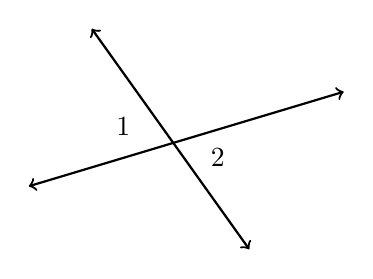
\begin{tikzpicture}[scale=.4]
        \draw [<->, thick] (0,-1.5)--(10,1.5);
        \draw [<->, thick] (2,3.5)--(7,-3.5);
        \node at (3,.4){1};
        \node at (6,-.6){2};
        %\draw [fill] (0,0) circle [radius=0.05] node[below]{$P$};
        %\draw [fill] (6,0) circle [radius=0.05] node[below]{$R$};
        %\draw [fill] (3,0) circle [radius=0.05] node[below]{$Q$};
      \end{tikzpicture}
      \end{flushright}

  \item Given $\overrightarrow{BA} \perp \overrightarrow{BC}$, $m \angle ABD = 2x-5$, and $m \angle DBC = x-10$. Find $m \angle DBC$. \\[0.5cm]
  For full credit, show the check using both angle measures.
    \begin{flushleft}
    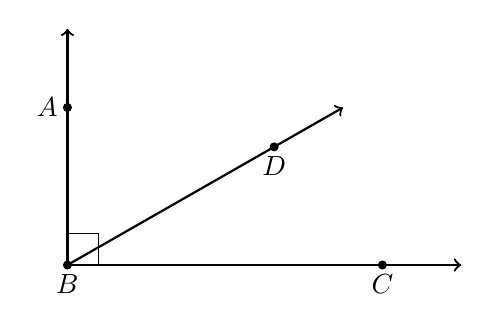
\begin{tikzpicture}[scale=1]
      \draw [<->, thick] (0,3)--(0,0)--(5,0);
      \draw [->, thick] (0,0)--(3.5, 2);
      \draw [-, thin] (0, 0.4)--(0.4, 0.4)--(0.4, 0);
      %\node at (3,.4){1};
      %\node at (6,-.6){2};
      \draw [fill] (0,0) circle [radius=0.05] node[below]{$B$};
      \draw [fill] (0,2) circle [radius=0.05] node[left]{$A$};
      \draw [fill] (4,0) circle [radius=0.05] node[below]{$C$};
      \draw [fill] (2.625, 1.5) circle [radius=0.05] node[below]{$D$};
    \end{tikzpicture}
    \end{flushleft}
    \vspace{6cm}

\subsubsection*{Midpoints: graphing, ratio partitions, solve for endpoint}

  \item Given $C(1,-2)$ and $D(7,9)$, find the coordinates of the midpoint of $\overline{CD}$, the point $M$.
    \vspace{4cm}

  \item Given $\overline{ABC}$, $AC=15$, and the point $B$ partitions $\overline{AC}$ in a ratio of 2:3.\\[0.5cm] Find ${AB}$. \\[1.5cm]
      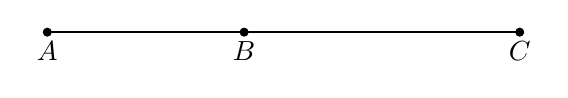
\begin{tikzpicture}
        \draw [-, thick] (1,0)--(7,0);
        \draw [fill] (1,0) circle [radius=0.05] node[below]{$A$};
        \draw [fill] (3.5,0) circle [radius=0.05] node[below]{$B$};
        \draw [fill] (7,0) circle [radius=0.05] node[below]{$C$};
      \end{tikzpicture} \vspace{3cm}

  \item Given $\overleftrightarrow{QS}$ as shown on the number line, with $Q$ having the coordinate 2.55 and $S$ the coordinate 5.23. \\[10pt] % Midpoint
    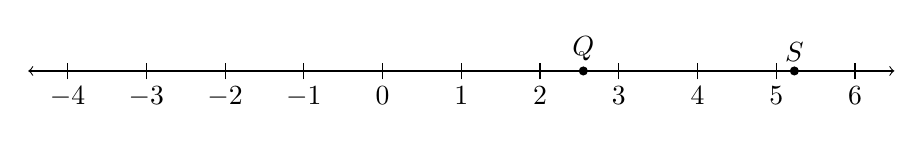
\begin{tikzpicture}
      \draw [<->] (-4.5,0)--(6.5,0);
      \foreach \x in {-4,...,6} %2 leading for diff!=1
        \draw[shift={(\x,0)},color=black] (0pt,-3pt) -- (0pt,3pt) node[below=5pt]  {$\x$};
        \draw [fill] (2.55,0) circle [radius=0.05] node[above] {$Q$};
        \draw [fill] (5.23,0) circle [radius=0.05] node[above] {$S$};
    \end{tikzpicture} \bigskip
    \begin{enumerate}
      \item Find the value of the coordinate of the point $R$, the midpoint of $\overline{QS}$. \vspace{4cm}
      \item The point $P$ is collinear with $\overleftrightarrow{QS}$ such that $Q$ is the midpoint of $\overleftrightarrow{PS}$. Mark $P$ on the line and state the value of its coordinate.
    \end{enumerate}\vspace{4cm}

\subsubsection*{Distance, areas, and perimeters: formulas, solving for dimensions}

  \item Given the square $BECA$ with $BE=2.50$.
    \begin{enumerate}
      \item Find the area of $BECA$. \vspace{2cm}
      \item Find the perimeter of $BECA$. \vspace{2cm}
    \end{enumerate}

  \item Given $P(-2,4)$ and $Q(1,0)$, find the length of $\overline{PQ}$.
      \vspace{5cm}

  \item Given $B(-7, 4)$, $U(5, -1)$, and $Z(-7, -1)$.
  \begin{enumerate}
    \item Plot and label the points on the graph, drawing $\overline{BU}$
    \item Draw the legs of the right triangle, $\overline{BZ}$ and $\overline{ZU}$, marking their lengths.
    \item Write down the distance formula for $BU$, substituting coordinate values.
    \item Find the value of $BU$.
  \end{enumerate}
  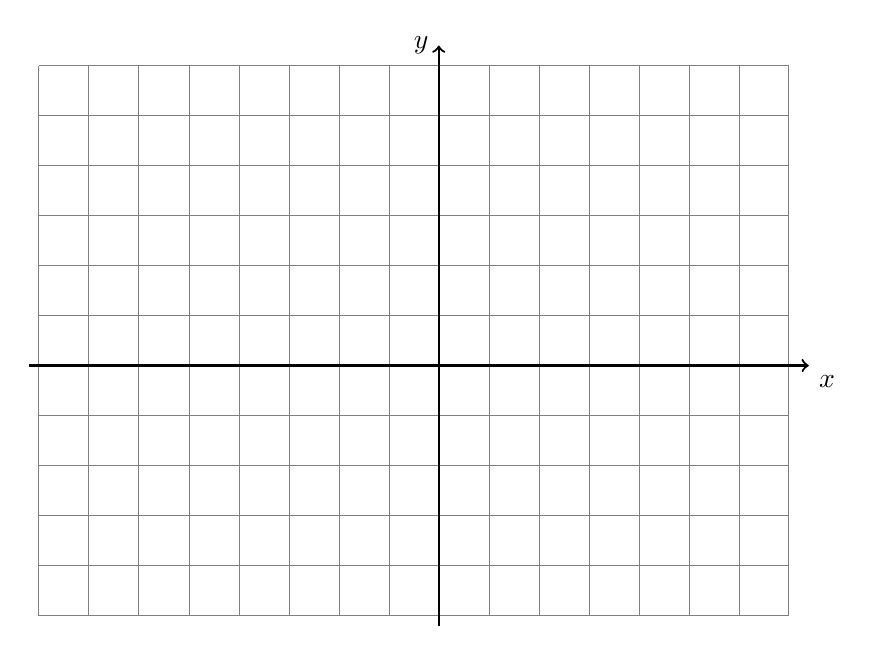
\begin{tikzpicture}[scale=.635]
    \draw [help lines] (-8,-5) grid (7,6);
    \draw [thick, ->] (-8.2,0) -- (7.4,0) node [below right] {$x$};
    \draw [thick, ->] (0,-5.2)--(0,6.4) node [left] {$y$};
  \end{tikzpicture}

  \item Given the circle $C$ with circumference $10\pi$. Find the area of $C$. \vspace{5cm}

\newpage
\subsubsection*{Constructions: aim for fluency}
  \item Construct an equilateral triangle with one side the given line segment $\overline{AB}$.
  \item Construction a perpendicular bisector of the given line segment, $\overline{GH}$.
  \item Construct an angle bisector of the given angle.

  \item Spicy: Construct the angle bisectors of the angles of the triangle and their intersection, the incenter.

\subsubsection*{Proof: Identify properties and know vocabulary}

  \item In a proof, each of the following statements are written. Write down the reason that would justify each step. \bigskip
    \begin{enumerate}
      \item $2(DE + FG)=2DE+2FG$  \hspace{0.6cm} $\rule{5cm}{0.15mm}$ property \bigskip
      \item $\overline{EF} \cong \overline{EF}$ \hspace{4cm} $\rule{5cm}{0.15mm}$ property \bigskip
      \item $DE+EF= FG+EF$  \hspace{1.7cm} $\rule{5cm}{0.15mm}$ property
    \end{enumerate}


  \end{enumerate}

\end{document}
